\documentclass{article}
\usepackage[a4paper, paperwidth=25cm, paperheight=25.5cm, left=1.5cm, right=1.5cm, top=1cm, bottom=2cm]{geometry}
\usepackage{tikz,tcolorbox}
\usepackage{amsmath}
\usepackage[table,xcdraw]{xcolor}
\usepackage{listings}
\usepackage{array,multirow} % For customizing tables
\usepackage{booktabs} % For better horizontal lines
\usepackage{makecell}
\setlength{\parindent}{0pt}
\usepackage{siunitx}
\usepackage{tkz-tab}
\usepackage{amssymb}
\usepackage{amsmath}
\usepackage{enumitem}



\newcommand{\exer}[1]{
  \section*{Exercice #1}
  \vspace{-0.5cm}
  \noindent\rule{\textwidth}{0.5pt}%
}

\newcommand{\tit}[1]{
\begin{center}
    \Large{\textbf{{#1}}}
\end{center}
}

\definecolor{commentgray}{HTML}{676160}
\definecolor{messagegreen}{HTML}{17B867}
\definecolor{myblue}{HTML}{10C2C4}

\tcbuselibrary{skins, breakable, theorems}


\newtcolorbox{prettyBox}[2]{
  enhanced,
  colback=white!90!#2,   % Background color based on the second parameter (color)
  colframe=#2!60!black,  % Frame color based on the second parameter (color)
  coltitle=white,        % Title color (white)
  fonttitle=\bfseries\Large,
  title=#1,              % Title from the first parameter
  boxrule=1mm,
  arc=0.5mm,
  drop shadow=#2!35!gray, % Drop shadow color based on the second parameter (color)
}

\lstdefinestyle{pythonstyle}{
    language=python,                    % Language set to Python
    basicstyle=\ttfamily\footnotesize,   % Change basic font size
    keywordstyle=\color{blue}\bfseries, % Different keyword style
    stringstyle=\color{red},         % Different string color
    commentstyle=\color{green!60!black}\itshape, % Adjust comment color
    numbers=left,                       % Line numbers on the left
    numberstyle=\tiny\color{gray},      % Smaller number font and color
    stepnumber=1,                       % Number each line
    frame=single,                       % Single frame around code
    tabsize=4,                          % Adjust tab size
    showstringspaces=false,             % Do not show spaces in strings
    captionpos=b,% Position of caption
    breaklines=true,
    inputencoding=utf8
}




\begin{document}
\tit{TP N\(^{\boldsymbol{\circ}}\)\hspace{0.1cm}1}
\exer{1}


\textbf{\underline{ex1.html}}
\vspace{0.1cm}

\lstinputlisting[style=htmlstyle]{Code/EX1/ex1.html}

\vspace{1.5cm}

\textbf{\underline{Output}}

\vspace{0.1cm}
\begin{center}
\setlength{\fboxrule}{2pt} % Set border thickness
\fbox{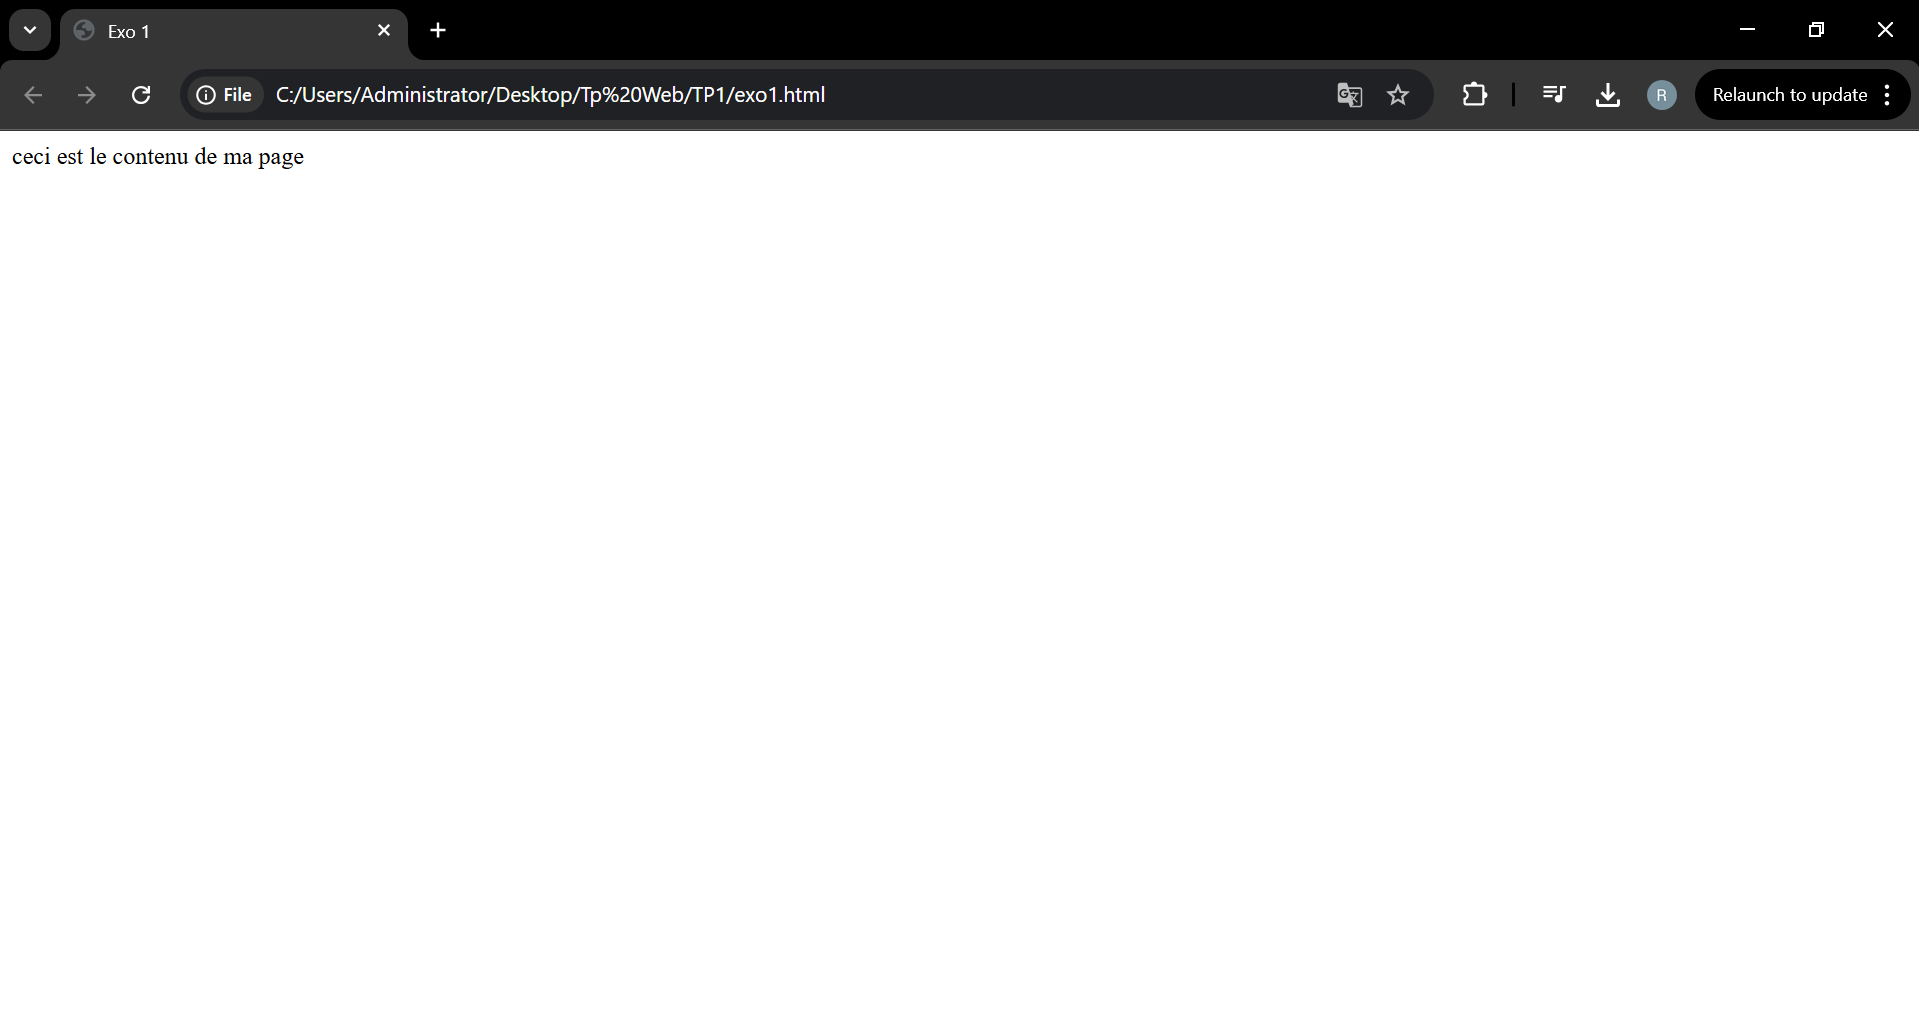
\includegraphics[height=0.4\textheight]{Code/EX1/ex1.PNG}}
\end{center}

\newpage
\begin{center}
    \Huge{\textbf{\underline{Exercise 2}}}
\end{center}

\vspace{0.45cm}

Give the implementation for an application that creates only one
instance of the pilot with card code 100 using singleton.

\vspace{0.75cm}

\textbf{\underline{Solution}}\\[0.15cm]
\textbf{\underline{Java Code:}}
\vspace{0.1cm}
\lstinputlisting[style=javastyle]{Exercices/EX2/Pilot.java}

\vspace{0.5cm}
\lstinputlisting[style=javastyle]{Exercices/EX2/Main.java}

\vspace{1cm}

\textbf{\underline{Output:}}
\vspace{0.1cm}
\begin{lstlisting}[style=cmd]
Running on thread: Thread-0
Running on thread: Thread-1
Pilot Instance
Running on thread: Thread-2
\end{lstlisting}




\newpage
\exer{3}

\setcounter{section}{0}

\vspace{0.25cm}


\section{Import}
\begin{prettyBox}{Import}{myblue}
\begin{itemize}
    \item \texttt{numpy} : Les fonctions mathématiques prédéfinies, et \texttt{linspace} pour créer  
        les vecteur des coordonnées x de chaque fonctions.  
    \item \texttt{matplotlib} : Dessine les graphes.  
    \item \texttt{collections} : Crée une nouvelle structure avec \texttt{namedtuple}.  
\end{itemize}
\end{prettyBox}
\vspace{0.5cm}
\lstinputlisting[style=pythonstyle, firstline = 1,lastline=3,basicstyle= \ttfamily\scriptsize]{Exercices/EX3/ex3.py}

\vspace{1cm}

\section{Définition De La Fonction \(f\)}
\lstinputlisting[style=pythonstyle, firstline = 7,lastline=9,basicstyle= \ttfamily\scriptsize]{Exercices/EX3/ex3.py}

\vspace{1cm}
\section{\(\epsilon\)}
\lstinputlisting[style=pythonstyle, firstline = 71,lastline=71,basicstyle= \ttfamily\scriptsize]{Exercices/EX3/ex3.py}

\vspace{1cm}
\section{Génération Des Vecteurs}
\lstinputlisting[style=pythonstyle, firstline = 77,lastline=78,basicstyle= \ttfamily\scriptsize]{Exercices/EX3/ex3.py}

\newpage
\section{Nouvelle Structure root}
\begin{prettyBox}{root}{myblue}
On a créé une nouvelle structure en utilisant \texttt{namedtuple} root. Elle représente 
les racines pour \( f(x) = 0 \) et possède trois attributs :
\begin{itemize}
    \item \textbf{position} : coordonnée x de la racine
    \item \textbf{a} : extrémité gauche de l'intervalle auquel la racine appartient
    \item \textbf{b} : extrémité droite de l'intervalle auquel la racine appartient 
    \item \textbf{phi} : le label de la function point fixe \(\varphi\).
    \item \textbf{x\_0} : la valeur de depart \(x_0 \in [a,b]\).
    \item \textbf{eps} : la valeur de la tolerance\(\epsilon\).
    \item \textbf{error} : Estimation de l'erreur de la method dichotomie.
    \item \textbf{iteration}: Nombre d'iteration de la method dichotomie.
\end{itemize}
\end{prettyBox}
\vspace{0.5cm}
\lstinputlisting[style=pythonstyle, firstline = 5,lastline=5,basicstyle= \ttfamily\scriptsize]{Exercices/EX3/ex3.py}

\vspace{1cm}
\section{Trouver \(\varphi\) Pour \(f\) Sur [1,2]}
On a \(f(x) = x - 1 - e^{-x} \) et \([a,b] = [1,2]\)

\vspace{0.75cm}
\begin{center}
    \(x - 1 - e^{-x} = 0\)\\[0.1cm]
    \(\boxed{x  =   e^{-x} + 1  = \varphi}\)\\[0.1cm]
\end{center}

\vspace{0.5cm}
\textbf{\underline{\(\varphi'\)}}
\begin{center}
    \begin{align*}
        &\boxed{\varphi'(x) = - e^{-x} }\\[0.15cm]
        &\boxed{\forall x \hspace{0.4cm} \varphi' < 0}
    \end{align*}
\end{center}

\vspace{0.5cm}
\textbf{\underline{\(\varphi''\)}}
\begin{center}
    \begin{align*}
        &\boxed{\varphi''(x) =  e^{-x} }\\[0.15cm]
        &\boxed{\forall x \hspace{0.4cm} \varphi'' > 0}
    \end{align*}
\end{center}

\vspace{1cm}
\textbf{\underline{Variation Table}}

\begin{center}
 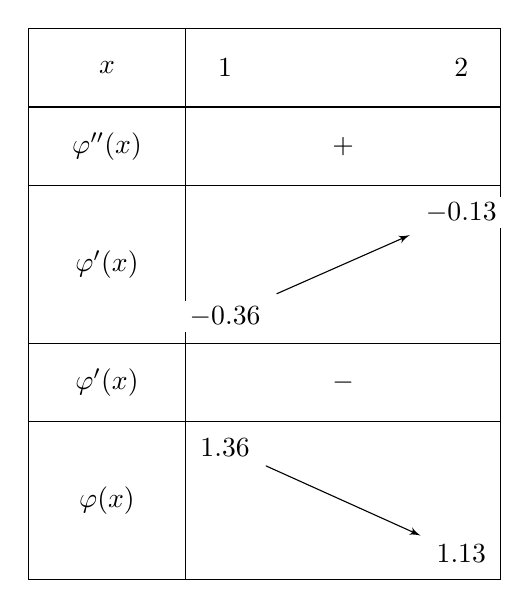
\begin{tikzpicture}
     \tkzTabInit {$x$/1, $\varphi''(x)$/1 , $\varphi'(x)$/2,$\varphi'(x)$/1,$\varphi(x)$/2}
     {$1$, $2$}
    \tkzTabLine{,+,}
    \tkzTabVar{-/$-0.36$ , +/$-0.13$ }
    \tkzTabLine{,-,}
    \tkzTabVar{+/$1.36$ , -/$1.13$ }
\end{tikzpicture}
\end{center}
\vspace{0.75cm}


\(\varphi([1,2]) \subseteq [1,2] \Longrightarrow \varphi\) est stable en \([1,2]\)\\[0.2cm]
\(\varphi \in C^{1} \text{  et } \displaystyle\sup_{x \in [1, 2]} |\varphi'(x)| = 0.36 < 1 \Longrightarrow \varphi\) est contractante en \([1,2]\)


\vspace{1.25cm}
\textbf{Conclusion :}
\vspace{-0.25cm}
\begin{center}
    \(\boxed{\varphi = e^{-x} + 1 \hspace{0.25cm},\hspace{0.25cm} k = 0.36}\)
\end{center}

\newpage
\section{Implementation De La Method Point-Fixe}
\subsection{Estimation De L'erreur}
\lstinputlisting[style=pythonstyle, firstline = 14,lastline=15,basicstyle= \ttfamily\scriptsize]{Exercices/EX3/ex3.py}

\vspace{0.5cm}
\subsection{Definition De La Fonction \(\varphi\)}
\lstinputlisting[style=pythonstyle, firstline = 10,lastline=11,basicstyle= \ttfamily\scriptsize]{Exercices/EX3/ex3.py}

\vspace{0.5cm}
\subsection{Initialisation Des Variables}
\lstinputlisting[style=pythonstyle, firstline = 72,lastline=75,basicstyle= \ttfamily\scriptsize]{Exercices/EX3/ex3.py}

\vspace{0.5cm}
\subsection{Algorithm De Point-Fixe}
\lstinputlisting[style=pythonstyle, firstline = 18,lastline=41,basicstyle= \ttfamily\scriptsize]{Exercices/EX3/ex3.py}

\newpage
\section{Dessiner}
\subsection{Scatter}
\lstinputlisting[style=pythonstyle, firstline = 44,lastline=50,basicstyle= \ttfamily\scriptsize]{Exercices/EX3/ex3.py}
\vspace{0.5cm}

\subsection{Graphe \& Table }
\lstinputlisting[style=pythonstyle, firstline = 54,lastline=68,basicstyle= \ttfamily\scriptsize]{Exercices/EX3/ex3.py}

\vspace{1cm}

\section{Rest Du Code}
\lstinputlisting[style=pythonstyle, firstline = 80,basicstyle= \ttfamily\scriptsize]{Exercices/EX3/ex3.py}

\vspace{1.5cm}
\section{Figure}

\begin{center}
    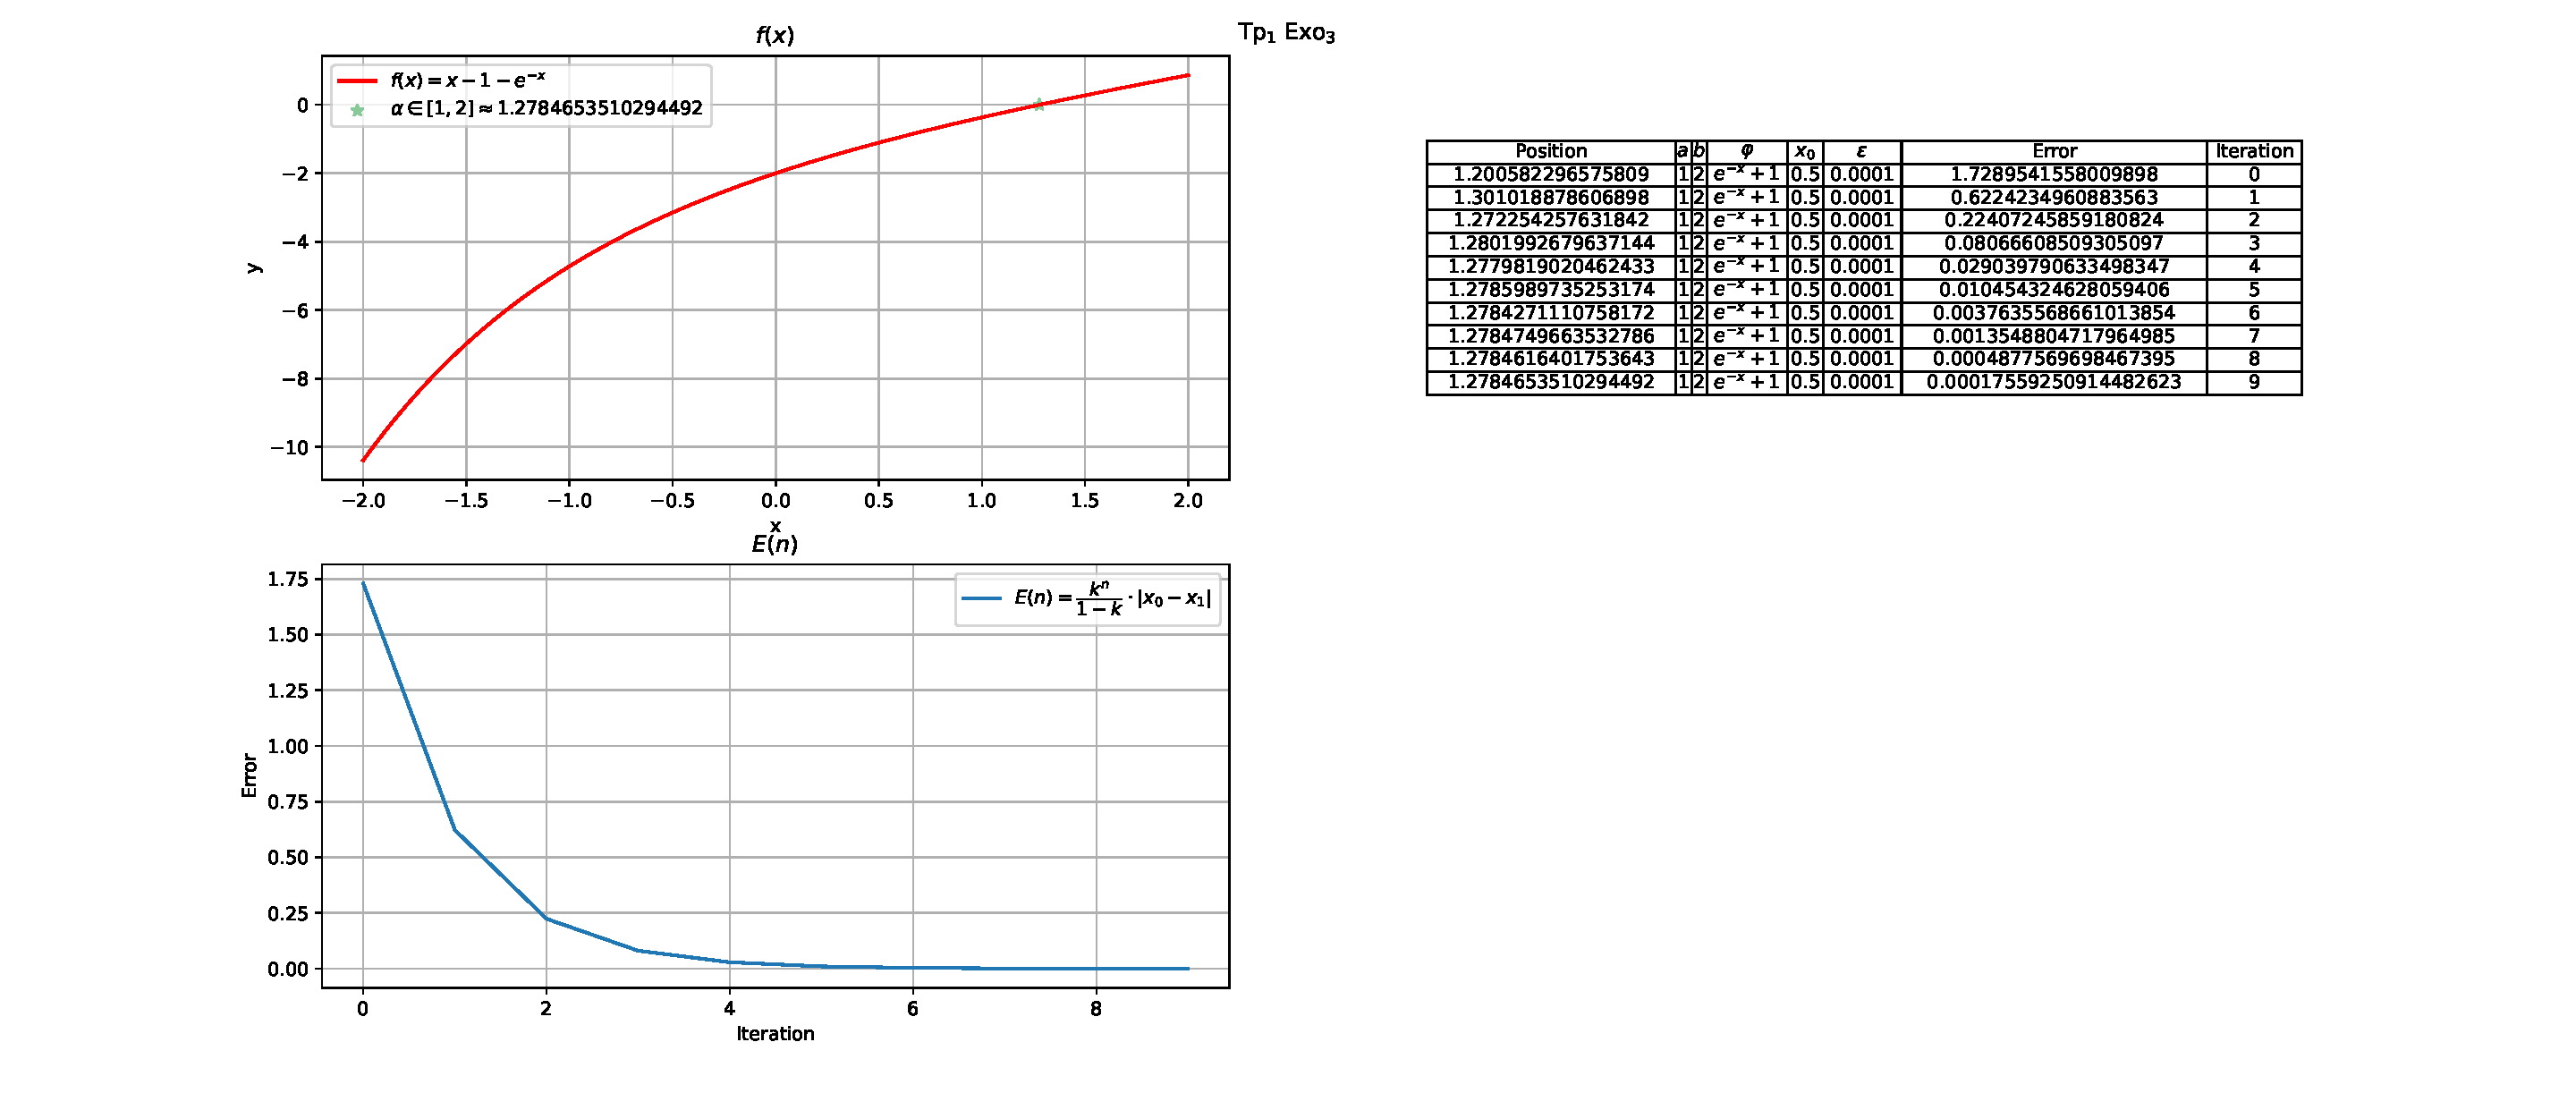
\includegraphics[height=0.35\textheight]{Exercices/EX3/fig.pdf}
\end{center}

\vspace{1cm}
\begin{prettyBox}{Remarque}{myblue}
On remarque que \(E(x)\) est decroissante et converge vers 0
\end{prettyBox}

\end{document}
